\chapter{Multiple Subplots\label{Ch31}}
Sometimes it is helpful to compare different views of data side by side. To this end,
Matplotlib has the concept of subplots: groups of smaller axes that can exist together
within a single figure. These subplots might be insets(画中画), grids of plots, or other more
complicated layouts. In this chapter we'll explore four routines for creating subplots
in Matplotlib.
\section{plt.axes: Subplots by Hand}
The most basic method of creating an axes is to use the plt.axes\marginpar[plt.axes]{plt.axes} function. As we've
seen previously, by default this creates a standard axes object that fills the entire figure. plt.axes also takes an optional argument that is a list of four numbers in the
figure coordinate system (\verb|[left, bottom, width, height]|), which ranges from 0 at
the bottom left of the figure to 1 at the top right of the figure.

For example, we might create an inset axes at the top-right corner of another axes by
setting the x and y position to 0.65 (that is, starting at 65\% of the width and 65% of
the height of the figure) and the x and y extents to 0.2 (that is, the size of the axes is
20\% of the width and 20\% of the height of the figure)(see \autoref{Example of an inset axes}).

The equivalent of this command within the object-oriented interface is \verb|fig.add_axes|\marginpar[fig.add\_axes]{fig.add\_axes}.
\begin{figure}
    \centering
    \begin{subfigure}[b]{.45\textwidth}
        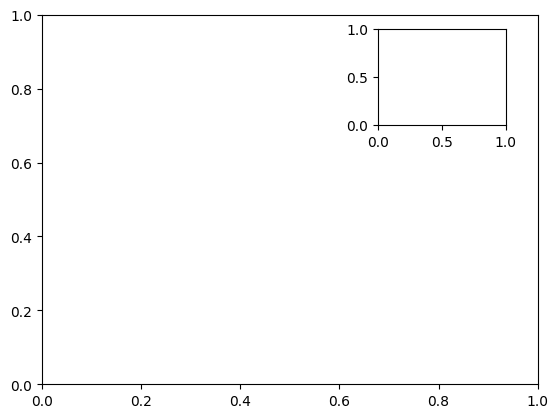
\includegraphics[width=\textwidth]{../img/Example of an inset axes.png}
        \caption{Example of an inset axes}
        \label{Example of an inset axes}
    \end{subfigure}
    \hfill
    \begin{subfigure}[b]{.45\textwidth}
        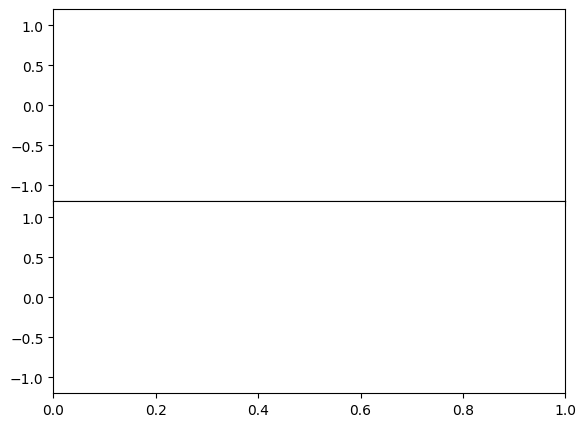
\includegraphics[width=\textwidth]{../img/Vertically stacked axes example.png}
        \caption{Vertically stacked axes example}
        \label{Vertically stacked axes example}
    \end{subfigure}
    \caption{Subplots by Hand}
\end{figure}
\section{plt.subplot: Simple Grids of Subplots}
Aligned columns or rows of subplots are a common enough need that Matplotlib has
several convenience routines that make them easy to create. The lowest level of these
is \verb|plt.subplot|\marginpar[plt.subplot]{plt.subplot}, which creates a single subplot within a grid. As you can see, this
command takes three integer arguments—the number of rows, the number of columns, and the index of the plot to be created in this scheme, which runs from the
upper left to the bottom right.(see \autoref{A plt.subplot example})

\begin{figure}
    \centering
    \begin{subfigure}[b]{.45\textwidth}
        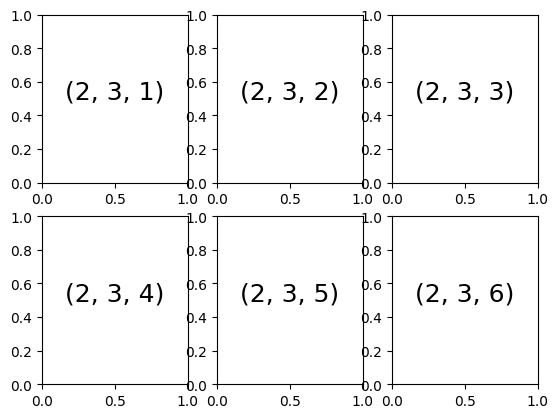
\includegraphics[width=\textwidth]{../img/A plt.subplot example.png}
        \caption{A plt.subplot example}
        \label{A plt.subplot example}
    \end{subfigure}
    \hfill
    \begin{subfigure}[b]{.45\textwidth}
        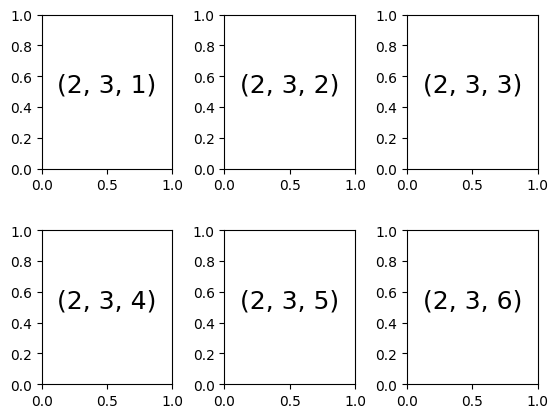
\includegraphics[width=\textwidth]{../img/plt.subplot with adjusted margins.png}
        \caption{plt.subplot with adjusted margins}
        \label{plt.subplot with adjusted margins}
    \end{subfigure}
    \caption{plt.subplot: Simple Grids of Subplots}
\end{figure}

The command \verb|plt.subplots_adjust| can be used to adjust the spacing between
these plots. The following code uses the equivalent object-oriented command,
\verb|fig.add_subplot|; \autoref{plt.subplot with adjusted margins} shows the result.

Here we've used the hspace and wspace arguments of \verb|plt.subplots_adjust|, which
specify the spacing along the height and width of the figure, in units of the subplot
size (in this case, the space is 40\% of the subplot width and height).
\section{plt.subplots: The Whole Grid in One Go}
The approach just described quickly becomes tedious when creating a large grid of
subplots, especially if you'd like to hide the x- and y-axis labels on the inner plots. For
this purpose, \verb|plt.subplots|\marginpar[plt.subplots]{plt.subplots} is the easier tool to use (note the s at the end of
subplots). Rather than creating a single subplot, this function creates a full grid of
subplots in a single line, returning them in a NumPy array. The arguments are the
number of rows and number of columns, along with optional keywords sharex and
sharey, which allow you to specify the relationships between different axes.

In comparison to plt.subplot, plt.subplots is more consistent with Python's conventional zero-based indexing, whereas plt.subplot uses MATLAB-style one-based
indexing.
\section{plt.GridSpec: More Complicated Arrangements}
To go beyond a regular grid to subplots that span multiple rows and columns,
\verb|plt.GridSpec|\marginpar[plt.GridSpec]{plt.GridSpec} is the best tool. plt.GridSpec does not create a plot by itself; it is
rather a convenient interface that is recognized by the plt.subplot command.

\begin{pyc}
    grid = plt.GridSpec(2, 3, wspace=.4, hspace=.3)
    plt.subplot(grid[0, 0])
    plt.subplot(grid[0, 1:])
    plt.subplot(grid[1, :2])
    plt.subplot(grid[1, 2])
    plt.show()
\end{pyc}

This type of flexible grid alignment has a wide range of uses. I most often use it when
creating multiaxes histogram plots.
\figures{Visualizing multidimensional distributions with plt.GridSpec}